% Options for packages loaded elsewhere
\PassOptionsToPackage{unicode}{hyperref}
\PassOptionsToPackage{hyphens}{url}
\PassOptionsToPackage{dvipsnames,svgnames*,x11names*}{xcolor}
%
\documentclass[
  11pt,
  a4paper,
]{article}
\usepackage{lmodern}
\usepackage{setspace}
\usepackage{amsmath}
\usepackage{ifxetex,ifluatex}
\ifnum 0\ifxetex 1\fi\ifluatex 1\fi=0 % if pdftex
  \usepackage[T1]{fontenc}
  \usepackage[utf8]{inputenc}
  \usepackage{textcomp} % provide euro and other symbols
  \usepackage{amssymb}
\else % if luatex or xetex
  \usepackage{unicode-math}
  \defaultfontfeatures{Scale=MatchLowercase}
  \defaultfontfeatures[\rmfamily]{Ligatures=TeX,Scale=1}
  \setmainfont[]{Arial}
\fi
% Use upquote if available, for straight quotes in verbatim environments
\IfFileExists{upquote.sty}{\usepackage{upquote}}{}
\IfFileExists{microtype.sty}{% use microtype if available
  \usepackage[]{microtype}
  \UseMicrotypeSet[protrusion]{basicmath} % disable protrusion for tt fonts
}{}
\makeatletter
\@ifundefined{KOMAClassName}{% if non-KOMA class
  \IfFileExists{parskip.sty}{%
    \usepackage{parskip}
  }{% else
    \setlength{\parindent}{0pt}
    \setlength{\parskip}{6pt plus 2pt minus 1pt}}
}{% if KOMA class
  \KOMAoptions{parskip=half}}
\makeatother
\usepackage{xcolor}
\IfFileExists{xurl.sty}{\usepackage{xurl}}{} % add URL line breaks if available
\IfFileExists{bookmark.sty}{\usepackage{bookmark}}{\usepackage{hyperref}}
\hypersetup{
  pdftitle={Análise de Resíduos em Modelos de Regressão Linear},
  pdfauthor={Francisco Piccolo},
  colorlinks=true,
  linkcolor=RoyalBlue,
  filecolor=Maroon,
  citecolor=Blue,
  urlcolor=RoyalBlue,
  pdfcreator={LaTeX via pandoc}}
\urlstyle{same} % disable monospaced font for URLs
\usepackage[margin=.5in]{geometry}
\usepackage{longtable,booktabs}
\usepackage{calc} % for calculating minipage widths
% Correct order of tables after \paragraph or \subparagraph
\usepackage{etoolbox}
\makeatletter
\patchcmd\longtable{\par}{\if@noskipsec\mbox{}\fi\par}{}{}
\makeatother
% Allow footnotes in longtable head/foot
\IfFileExists{footnotehyper.sty}{\usepackage{footnotehyper}}{\usepackage{footnote}}
\makesavenoteenv{longtable}
\usepackage{graphicx}
\makeatletter
\def\maxwidth{\ifdim\Gin@nat@width>\linewidth\linewidth\else\Gin@nat@width\fi}
\def\maxheight{\ifdim\Gin@nat@height>\textheight\textheight\else\Gin@nat@height\fi}
\makeatother
% Scale images if necessary, so that they will not overflow the page
% margins by default, and it is still possible to overwrite the defaults
% using explicit options in \includegraphics[width, height, ...]{}
\setkeys{Gin}{width=\maxwidth,height=\maxheight,keepaspectratio}
% Set default figure placement to htbp
\makeatletter
\def\fps@figure{htbp}
\makeatother
\setlength{\emergencystretch}{3em} % prevent overfull lines
\providecommand{\tightlist}{%
  \setlength{\itemsep}{0pt}\setlength{\parskip}{0pt}}
\setcounter{secnumdepth}{-\maxdimen} % remove section numbering
\pagestyle{plain}
\usepackage{lineno,sectsty,color,colortbl,titling} % add

% Left justification of the text: see https://www.sharelatex.com/learn/Text_alignment
% \usepackage[document]{ragged2e} % already in the latex template
\newcommand{\bleft}{\begin{flushleft}}
\newcommand{\eleft}{\end{flushleft}}
\allsectionsfont{\mdseries\bfseries\color{RoyalBlue}}
\pretitle{\begin{center}\LARGE\color{RoyalBlue}}
\usepackage{booktabs}
\usepackage{longtable}
\usepackage{array}
\usepackage{multirow}
\usepackage{wrapfig}
\usepackage{float}
\usepackage{colortbl}
\usepackage{pdflscape}
\usepackage{tabu}
\usepackage{threeparttable}
\usepackage{threeparttablex}
\usepackage[normalem]{ulem}
\usepackage{makecell}
\usepackage{xcolor}
\ifluatex
  \usepackage{selnolig}  % disable illegal ligatures
\fi

\title{Análise de Resíduos em Modelos de Regressão Linear}
\usepackage{etoolbox}
\makeatletter
\providecommand{\subtitle}[1]{% add subtitle to \maketitle
  \apptocmd{\@title}{\par {\large #1 \par}}{}{}
}
\makeatother
\subtitle{Testando Soluções com R}
\author{Francisco Piccolo}
\date{2019-09-05}

\begin{document}
\maketitle

\setstretch{1.2}
O modelo de regressão linear é bastante usado na predição de variáveis contínuas, onde há uma ou mais variáveis independentes buscando mapear o comportamento de uma variável dependente. O modelo é bastante simples e lembro ser um dos primeiros a ser ensinado nas aulas de econometria. Porém, apesar de sua simplicidade, é preciso se atentar a alguns detalhes sobre suas premissas para que os resultados deste modelo possam ser usados para a tomada de decisão.

Abaixo vou listar algumas das premissas da regressão linear:

\begin{enumerate}
\def\labelenumi{\roman{enumi})}
\item
  Ausência de multicolinearidade entre as variáveis independentes.
\item
  Ausência de autocorrelação na variável dependente.
\item
  Absence of pattern on the behavior of the model residuals, in other words, absence of heteroscedasticity.
\item
  Ausência de padrão no comportamento dos resíduos do modelo, ou seja, ausência de heterocedasticidade.
\item
  Resíduos se distribuem de acordo com uma distribuição normal.
\end{enumerate}

Tendo estas premissas atendidas, o modelo pode gerar conclusões confiáveis. Neste post eu vou desenvolver um modelo de regressão linear para testar as premissas \textbf{iii} e \textbf{iv} que tratam dos resíduos, para ver alguns casos práticos. O código usado neste post está nesta \href{https://github.com/FranciscoPiccolo/franciscopiccolo.github.io/blob/master/02.Posts_pdf/02.residual_analysis_in_econometric_models_20190905/article.Rmd}{pasta} do meu Github.

\hypertarget{exemplo-pruxe1tico-elasticidade-preuxe7o-x-oferta-na-produuxe7uxe3o-de-cana-de-auxe7uxfacar}{%
\subsubsection{Exemplo prático: Elasticidade preço x oferta na produção de cana de açúcar}\label{exemplo-pruxe1tico-elasticidade-preuxe7o-x-oferta-na-produuxe7uxe3o-de-cana-de-auxe7uxfacar}}

Este exemplo foi passado na minha aula de econometria em 2017. Na época o exercício foi realizado com o software \textbf{EViews}, por sorte eu guardei os dados e agora posso refazer o problema com mais facilidade com o uso do R. O dataset pode ser visualizado neste \href{https://github.com/FranciscoPiccolo/franciscopiccolo.github.io/blob/master/02.Posts_pdf/02.residual_analysis_in_econometric_models_20190905/datasets/dataset_1.csv}{link}.

No exercício, temos a variável independente (X) sendo o preço da cana de açúcar e a variável dependente (Y) sendo a área plantada de cana de açúcar (representando uma proxy para a oferta do produto). O objetivo deste modelo é tentar quantificar a elasticidade da oferta em função do preço, ou seja, quantificar quão sensível é a oferta da cana de açúcar quando ocorrem variações em seu preço.

Abaixo há uma amostragem do dataset.

\begin{table}[H]

\caption{\label{tab:unnamed-chunk-4}Amostra do Dataset}
\centering
\fontsize{10}{12}\selectfont
\begin{tabular}[t]{lrrr}
\toprule
\cellcolor{RoyalBlue}{\textcolor{white}{\textbf{ }}} & \cellcolor{RoyalBlue}{\textcolor{white}{\textbf{period}}} & \cellcolor{RoyalBlue}{\textcolor{white}{\textbf{area}}} & \cellcolor{RoyalBlue}{\textcolor{white}{\textbf{price}}}\\
\midrule
15 & 15 & 125 & 0.235821\\
\addlinespace
3 & 3 & 42 & 0.101075\\
\addlinespace
27 & 27 & 97 & 0.401437\\
\addlinespace
2 & 2 & 71 & 0.114894\\
\addlinespace
11 & 11 & 88 & 0.226087\\
\bottomrule
\end{tabular}
\end{table}

O modelo de regressão linear para este cenário será desenvolvido de acordo com a fórmula abaixo:

\[ lnY_t = \beta_0+\beta_1 (lnX_t) + \mu_t \]

Onde:

\(Y_t\) = Área plantada após a transformação com log natural (e)

\(X_t\) = Preço da cana de açúcar também após a transformação com log natural

\(\beta_0\) = Intercepto

\(\beta_1\) = Inclinação

\(\mu_t\) = Resíduos

Os dados precisam ter a aplicação do log natural, pois esta transformação faz com que as variações entre os períodos possam ser interpretadas como variações percentuais, e isso é necessário por conta de que a elasticidade é quantificada em termos percentuais. Esta característica ocorre apenas na transformação com logarítmo natural, se a transformação fosse feita com outros logs, a interpretação (de variaçõs percentuais) não seria válida.

O gráfico abaixo irá mostrar o comportamento das variáveis do dataset, bem como a curva de regressão linear, antes de aplicar a transformação log natural.

\begin{center}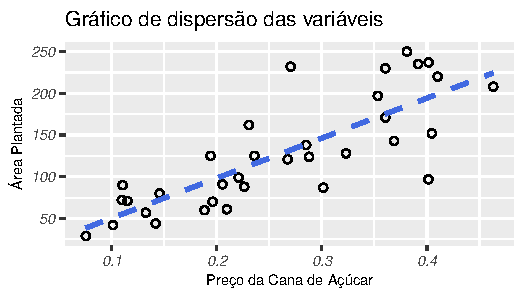
\includegraphics{article_files/figure-latex/unnamed-chunk-5-1} \end{center}

Podemos ver que há uma relação entre o preço do produto e sua oferta (área plantada). Agora vamos aplicar o log natural no modelo de regressão. Para isso, o R nos fornece duas opções:

\begin{itemize}
\item
  Ajustar as variáveis no dataset e construir o modelo usando as variáveis ajustadas.
\item
  Construir o modelo e indicar ``dentro dele'' que é necessário fazer a transformação antes de computar os resultados.
\end{itemize}

Vamos ver na prática como cada opção pode ser usada. O resultado final será idêntico.

Primeiro vou criar duas variáveis com os resultados dos dois métodos:

Com as duas variáveis criadas, vamos criar uma tabela comparando os principais resultados dos modelos:

\begin{table}[H]

\caption{\label{tab:unnamed-chunk-7}Comparativo dos Resultados}
\centering
\fontsize{10}{12}\selectfont
\begin{tabular}[t]{lrr}
\toprule
\cellcolor{RoyalBlue}{\textcolor{white}{\textbf{ }}} & \cellcolor{RoyalBlue}{\textcolor{white}{\textbf{X1º.Método}}} & \cellcolor{RoyalBlue}{\textcolor{white}{\textbf{X2º.Método}}}\\
\midrule
(Intercept) & 6.1113284 & 6.1113284\\
\addlinespace
price\_log & 0.9705823 & 0.9705823\\
\bottomrule
\end{tabular}
\end{table}

Conforme indicado, ambos os métodos geram o mesmo valor. Eu prefiro o segundo, que exige menos linhas de código. Com base nos coeficientes estimados, temos a seguinte equação:

\[\hat{Y} = 1.6416 + 0.9706X_1 + \mu\]
O resultado é estatisticamente significativo, visto que tanto o intercepto quanto a inclinação apresentam um valor-p baixo. Veja abaixo estes valores bem como o R².

\begin{longtable}[]{@{}ccccc@{}}
\toprule
\begin{minipage}[b]{(\columnwidth - 4\tabcolsep) * \real{0.25}}\centering
~\strut
\end{minipage} & \begin{minipage}[b]{(\columnwidth - 4\tabcolsep) * \real{0.15}}\centering
Estimate\strut
\end{minipage} & \begin{minipage}[b]{(\columnwidth - 4\tabcolsep) * \real{0.18}}\centering
Std. Error\strut
\end{minipage} & \begin{minipage}[b]{(\columnwidth - 4\tabcolsep) * \real{0.14}}\centering
t value\strut
\end{minipage} & \begin{minipage}[b]{(\columnwidth - 4\tabcolsep) * \real{0.17}}\centering
Pr(\textgreater\textbar t\textbar)\strut
\end{minipage}\tabularnewline
\midrule
\endhead
\begin{minipage}[t]{(\columnwidth - 4\tabcolsep) * \real{0.25}}\centering
\textbf{(Intercept)}\strut
\end{minipage} & \begin{minipage}[t]{(\columnwidth - 4\tabcolsep) * \real{0.15}}\centering
6.111\strut
\end{minipage} & \begin{minipage}[t]{(\columnwidth - 4\tabcolsep) * \real{0.18}}\centering
0.1686\strut
\end{minipage} & \begin{minipage}[t]{(\columnwidth - 4\tabcolsep) * \real{0.14}}\centering
36.25\strut
\end{minipage} & \begin{minipage}[t]{(\columnwidth - 4\tabcolsep) * \real{0.17}}\centering
1.468e-27\strut
\end{minipage}\tabularnewline
\begin{minipage}[t]{(\columnwidth - 4\tabcolsep) * \real{0.25}}\centering
\textbf{log(price)}\strut
\end{minipage} & \begin{minipage}[t]{(\columnwidth - 4\tabcolsep) * \real{0.15}}\centering
0.9706\strut
\end{minipage} & \begin{minipage}[t]{(\columnwidth - 4\tabcolsep) * \real{0.18}}\centering
0.1106\strut
\end{minipage} & \begin{minipage}[t]{(\columnwidth - 4\tabcolsep) * \real{0.14}}\centering
8.773\strut
\end{minipage} & \begin{minipage}[t]{(\columnwidth - 4\tabcolsep) * \real{0.17}}\centering
5.031e-10\strut
\end{minipage}\tabularnewline
\bottomrule
\end{longtable}

\begin{longtable}[]{@{}cccc@{}}
\caption{Fitting linear model: log(area) \textasciitilde{} log(price)}\tabularnewline
\toprule
\begin{minipage}[b]{(\columnwidth - 3\tabcolsep) * \real{0.21}}\centering
Observations\strut
\end{minipage} & \begin{minipage}[b]{(\columnwidth - 3\tabcolsep) * \real{0.31}}\centering
Residual Std. Error\strut
\end{minipage} & \begin{minipage}[b]{(\columnwidth - 3\tabcolsep) * \real{0.12}}\centering
\(R^2\)\strut
\end{minipage} & \begin{minipage}[b]{(\columnwidth - 3\tabcolsep) * \real{0.24}}\centering
Adjusted \(R^2\)\strut
\end{minipage}\tabularnewline
\midrule
\endfirsthead
\toprule
\begin{minipage}[b]{(\columnwidth - 3\tabcolsep) * \real{0.21}}\centering
Observations\strut
\end{minipage} & \begin{minipage}[b]{(\columnwidth - 3\tabcolsep) * \real{0.31}}\centering
Residual Std. Error\strut
\end{minipage} & \begin{minipage}[b]{(\columnwidth - 3\tabcolsep) * \real{0.12}}\centering
\(R^2\)\strut
\end{minipage} & \begin{minipage}[b]{(\columnwidth - 3\tabcolsep) * \real{0.24}}\centering
Adjusted \(R^2\)\strut
\end{minipage}\tabularnewline
\midrule
\endhead
\begin{minipage}[t]{(\columnwidth - 3\tabcolsep) * \real{0.21}}\centering
34\strut
\end{minipage} & \begin{minipage}[t]{(\columnwidth - 3\tabcolsep) * \real{0.31}}\centering
0.3088\strut
\end{minipage} & \begin{minipage}[t]{(\columnwidth - 3\tabcolsep) * \real{0.12}}\centering
0.7063\strut
\end{minipage} & \begin{minipage}[t]{(\columnwidth - 3\tabcolsep) * \real{0.24}}\centering
0.6972\strut
\end{minipage}\tabularnewline
\bottomrule
\end{longtable}

Embora o modelo consiga explicar \textasciitilde70\% da variação na variável dependente, é preciso analisar os reíduos gerados para poder ter confiança no resultado e fazer projeções (objetivo principal). No gráfico abaixo, vamos ver como se distribui os resíduos do modelo em um Histograma e Gráfico QQ (quantile-quantile)

\begin{center}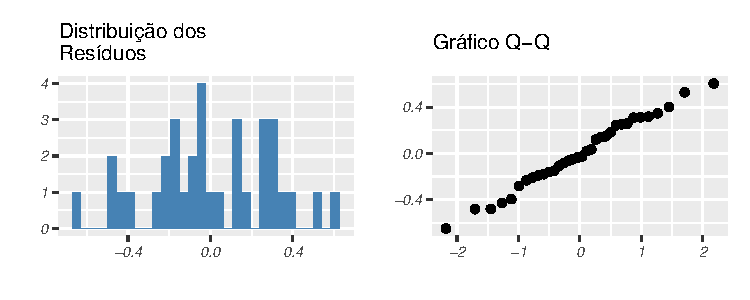
\includegraphics{article_files/figure-latex/unnamed-chunk-10-1} \end{center}

Ambos os gráficos indicam distribuição normal dos resíduos. Apesar desta forma visual ser recomendada, as vezes ela não é suficiente, casos em que o pesquisador precisará usar métodos mais formais para gerar uma conclusão. Para validação da independência no comportamento dos resíduos pode-se usar o teste \textbf{Durbin Watson}. O código abaixo realiza este teste.

\begin{longtable}[]{@{}ccc@{}}
\caption{Durbin-Watson test: \texttt{df\ \%\textgreater{}\%\ lm(formula\ =\ log(area)\ \textasciitilde{}\ log(price))}}\tabularnewline
\toprule
\begin{minipage}[b]{(\columnwidth - 2\tabcolsep) * \real{0.24}}\centering
Test statistic\strut
\end{minipage} & \begin{minipage}[b]{(\columnwidth - 2\tabcolsep) * \real{0.21}}\centering
P value\strut
\end{minipage} & \begin{minipage}[b]{(\columnwidth - 2\tabcolsep) * \real{0.36}}\centering
Alternative hypothesis\strut
\end{minipage}\tabularnewline
\midrule
\endfirsthead
\toprule
\begin{minipage}[b]{(\columnwidth - 2\tabcolsep) * \real{0.24}}\centering
Test statistic\strut
\end{minipage} & \begin{minipage}[b]{(\columnwidth - 2\tabcolsep) * \real{0.21}}\centering
P value\strut
\end{minipage} & \begin{minipage}[b]{(\columnwidth - 2\tabcolsep) * \real{0.36}}\centering
Alternative hypothesis\strut
\end{minipage}\tabularnewline
\midrule
\endhead
\begin{minipage}[t]{(\columnwidth - 2\tabcolsep) * \real{0.24}}\centering
1.291\strut
\end{minipage} & \begin{minipage}[t]{(\columnwidth - 2\tabcolsep) * \real{0.21}}\centering
0.009801 * *\strut
\end{minipage} & \begin{minipage}[t]{(\columnwidth - 2\tabcolsep) * \real{0.36}}\centering
true autocorrelation is
greater than 0\strut
\end{minipage}\tabularnewline
\bottomrule
\end{longtable}

O resultado do teste foi de 1.2912, mas apenas com este valor não é possível fazer uma conclusão. Em conjunto com este valor é preciso saber os valores limiares \textbf{DL} e \textbf{DU}, que podem ser encontrados nesta \href{http://www.portalaction.com.br/analise-de-regressao/33-diagnostico-de-independencia}{tabela}. Para encontrar os valores com nesta tabela, basta saber o número de observações no dataset (i.e.~33), o nível de significância do teste (i.e.~0.05) e os graus de liberdade (i.e.~1). Com isso, tem-se:

\textbf{DL} = 1.35

\textbf{DU} = 1.49

Tendo DW igual a 1.2912, acima de 0 e abaixo de DL, pode-se concluir que os resíduos são independentes.

Com isso, podemos concluir que de fato o modelo é confiável para realizar projeções, pois tanto os gráficos quanto o teste formal indicam que as premissas (iii) e (iv) estão sendo atendidas. Desta forma, podemos concluir que há elasticidade na oferta de cana de açúcar com relação ao seu preço.

\end{document}
